\section{Background for Experiments}

\subsection{Superpixel}
\label{sec:superpixel}

\begin{figure}[t]
  \centering
  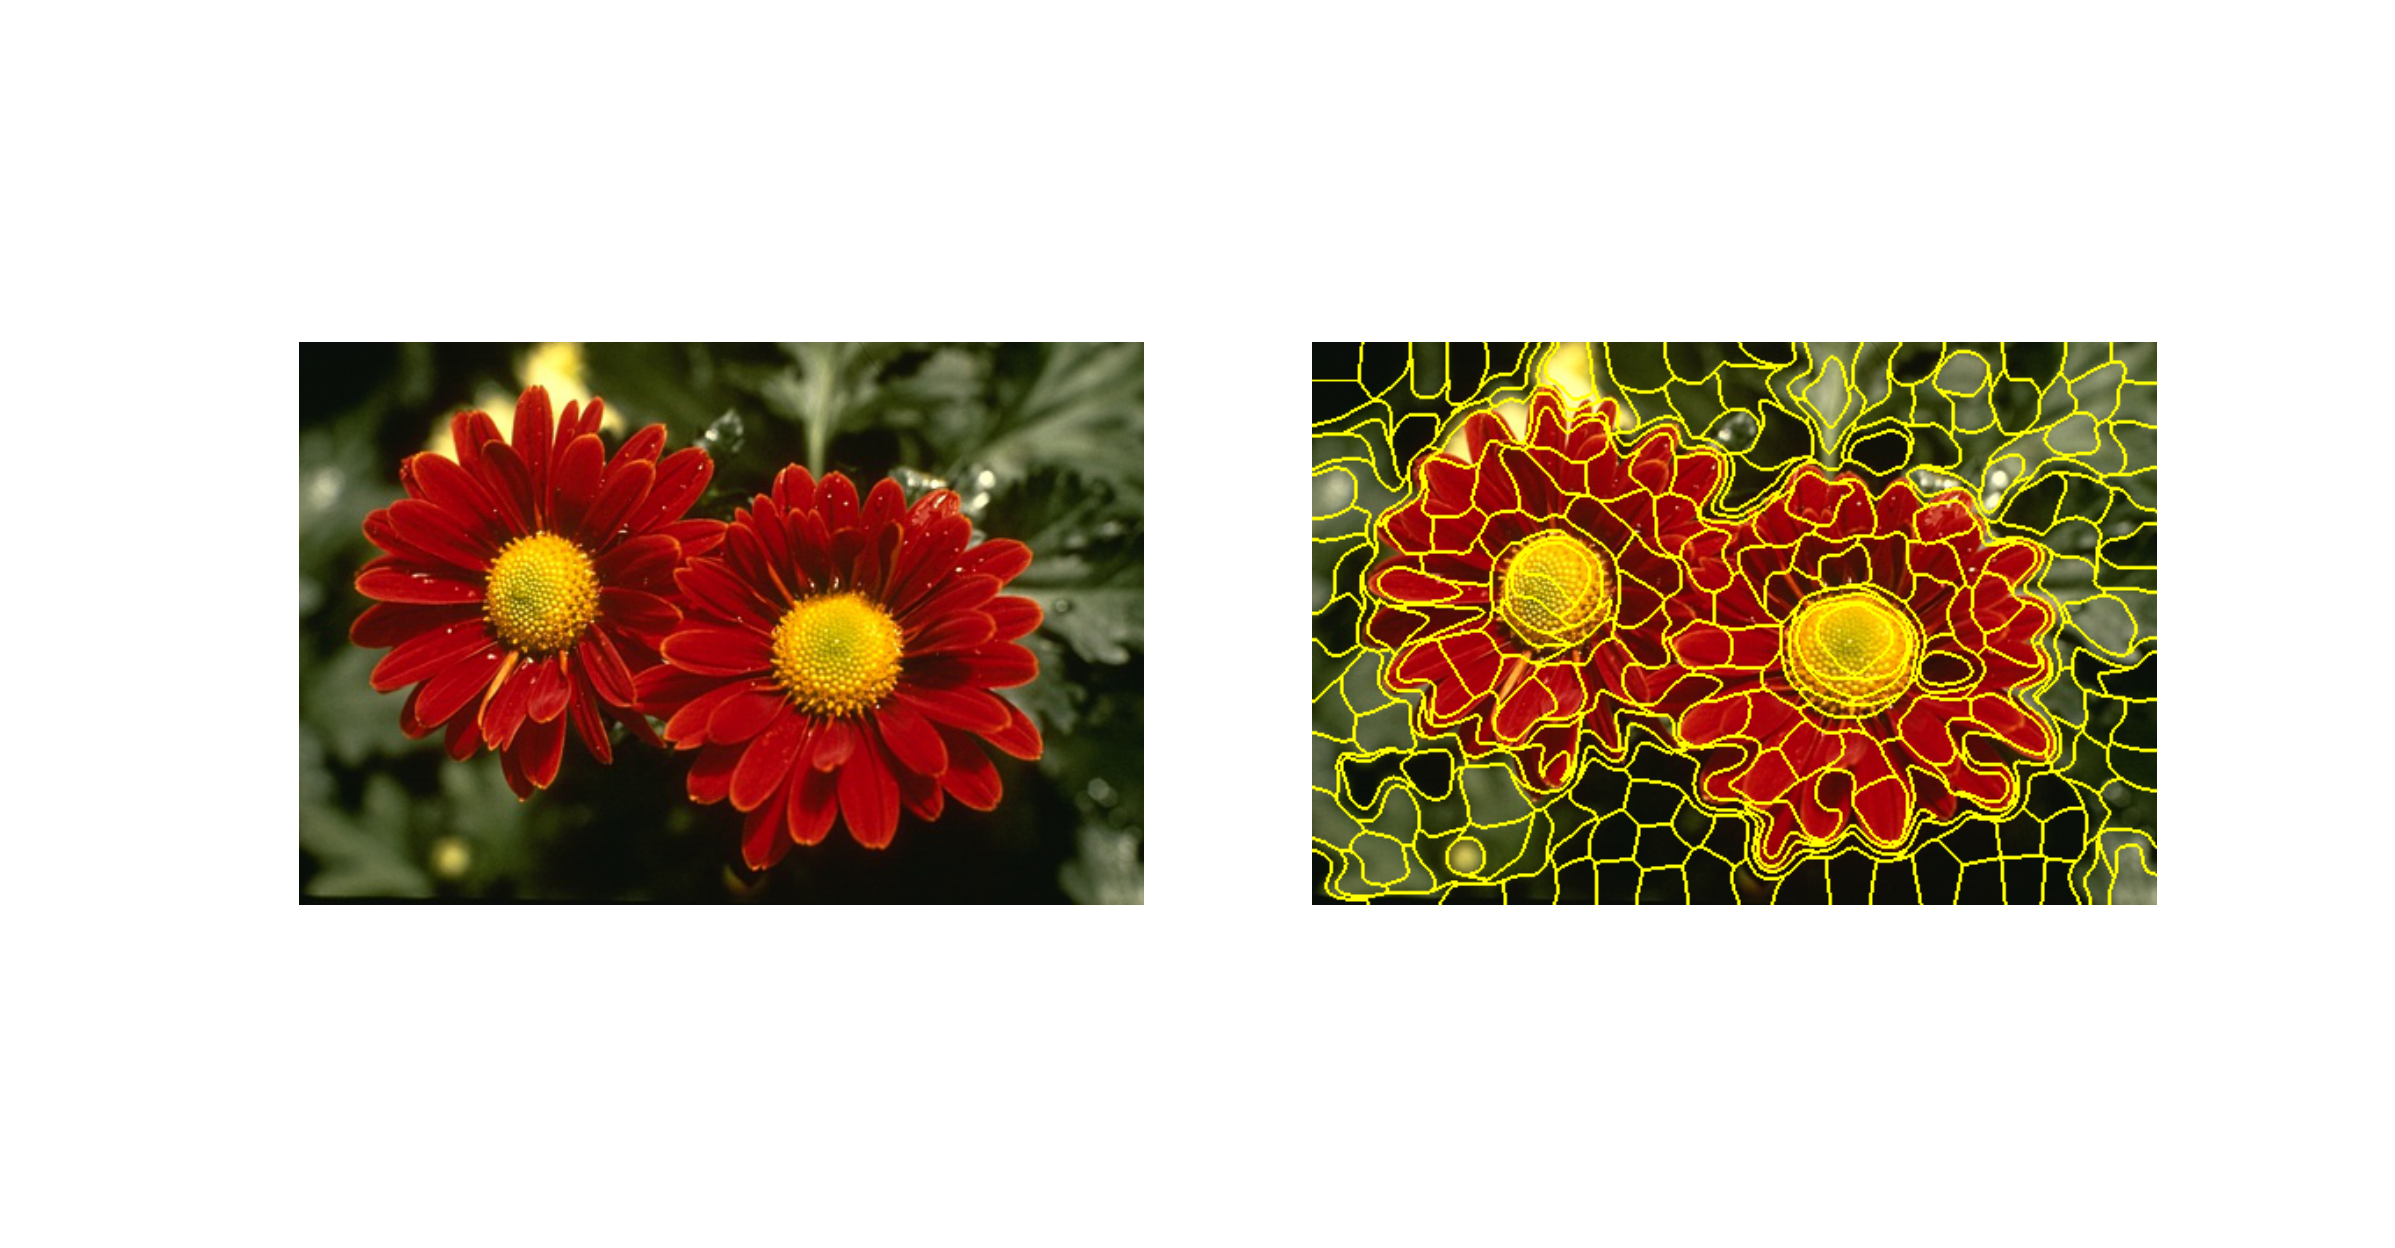
\includegraphics[width=1\linewidth]{RelatedWorks/figures/Flower_Origin_Segment.png}
  \caption{\label{fig:superpixel_example} Picture on the left is
    the original picture which contains 154,400 pixels. Picture
    on the right is the same picture represented by 268 superpixels}
\end{figure}

Markov Random Fields are often defined on grids of pixels or
``cliques''. However, artificial pixel-grids are usually
computational expensive and not natrual representations of
images. A much preferable representation is to group images in a
both perceptual and semantic meaningful way. Superpixel
algorithms, by capturing redundancy in images, can group pixels
into semantically meaningful homogeneous regions and reduce
hundreds of thousands of pixels into several hundreds of
superpixels (see figure~\ref{fig:superpixel_example}). Such a superpixel map can greatly increase the
efficiency of images processing tasks by providing an efficient
primitive on which MRF can compute
Energies\cite{achanta2012slic}.

There are various superpixel segmentation algorithms. When
choosing the desirable algorithm we mainly consider the following
two aspects\cite{achanta2012slic}:

\begin{enumerate}
\item Computational Efficiency: Superpixels should be fast to
  generate. Algorithms with less complexity are much preferable.
\item Adherence to boundaries: Algorithms which can generate
  superpixels with higher boundary recall (less true edges are
  missed) are much preferable.
\end{enumerate}

Basing on those two considerations the superpixel algorithm we use
in this thesis is the state-of-the-art \emph{Simple Linear
  Iterative Clustering} (SLIC) algorithm which out-performs other
algorithms in nearly all aspects\cite{achanta2012slic}. SLIC in
essence is an adaptation of $k$-means clustering algorithm. It
mainly differs from $k$-means with two
distinctions\cite{achanta2012slic}:

\begin{figure*}[h]
    \centering
    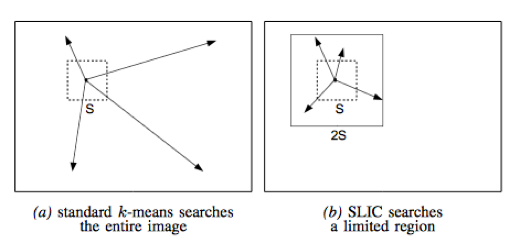
\includegraphics[width=0.8\linewidth]{RelatedWorks/figures/SLIC_AssignStep.png}
    \caption{\label{fig:SLIC_Regions}SLIC narrows the superpixel
      search regions.}
\end{figure*}

\begin{enumerate}
\item Searching space: In the assignment step $k$-means
  clustering computes distances from each cluster to every pixel
  in the image. On the other hand SLIC narrow the search space
  into a $2S\times 2S$ region (see figure~\ref{fig:SLIC_Regions}), where $S=\sqrt{\frac{N}{K}}$. $N$
  is the number of total pixels in images and $k$ is the only
  parameter of the algorithm which defines the number of
  superpixels (clusterings). Therefore, the SLIC algorithm
  reduces the complexity from $k$-means' $\mathcal{O}(N^k)$ to a
  linear complexity $\mathcal{O}(N)$.

\item Distance measurement: Distance in $k$-means algorithm is
  measured by Euclidean norm of color vectors between pairs of
  pixels. SLIC algorithm also takes spatial distance into account
  by redefining the distance as $D =
  \sqrt{d_c^2+(\frac{d_s}{S})^2m^2}$ where $d_c$ is the Euclidean
  norm of color vectors and $d_s$ is the Euclidean norm of pixels'
  positions. $m$ is a constant which indicates the relative
  importance between color distance and spatial distance and thus
  balances the compactness and adherence to boundries in
  generated superpixels.
\end{enumerate}

In this thesis we use SLIC as our cliques generating algorithm
because it is fast to compute and out-performs other algorithms
on adherence to image boundries while keeping results compact.

\subsection{GrabCut}
\label{sec:grabcut}

\begin{figure}[b]
  \centering
  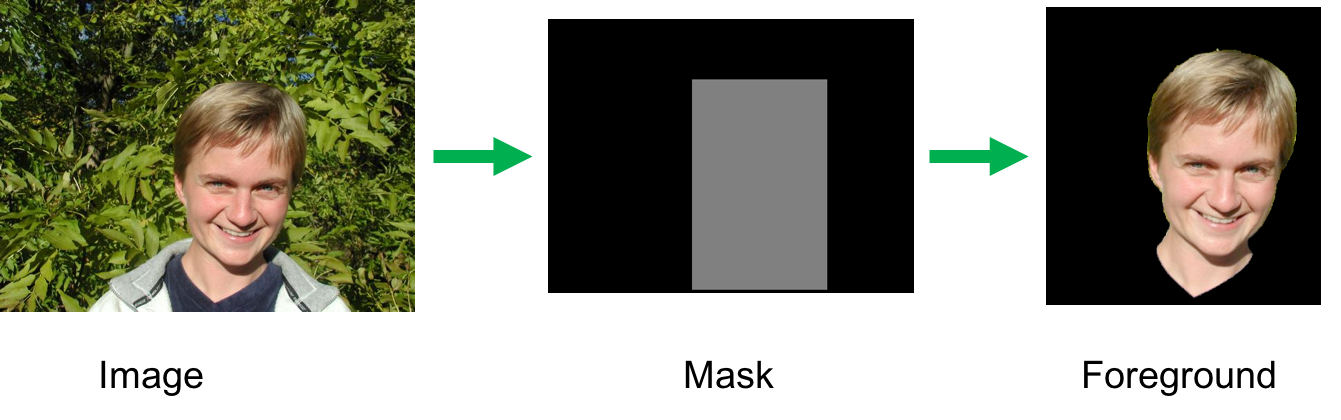
\includegraphics[width=1\linewidth]{RelatedWorks/figures/grabcut_task.png}
  \caption{\label{fig:grabcut_example} Picture on the left is
    the original picture. Picture
    on the middle is a user defined mask. The task is to extract
    foreground pixels within that rectangle. On the right is the
    ground truth foreground.}
\end{figure}

\emph{GrabCut} algorithm was proposed
by~\citename{Rother:SIGGRAPH04} in order to solve background
foreground segmentation problem (see figure~\ref{fig:grabcut_example}). They first defined MRFs over an
labeled image and then use \emph{graph-cuts}~\cite{Boykov:ICCV01} method to do the
inference. In this section we mainly focus on two of their
contributions: estimating color distribution (foreground and
background) using \emph{Gaussian Mixture Models} (GMMs) and an
\emph{EM} like two-step algorithm to train their model.

Suppose there are $N$ pixels in an image. In order to construct
MRFs, they first defined an energy
function~\eqref{eq:energyfunction_UPH} with unary and pairwise
terms:

\begin{align}
  \label{eq:grabcut_energy}
  E(\alpha, \bk, \btheta, \bz) = 
  \sum_{i\in \N}{\phi^U(\alpha_i, \bk_i, \btheta, \bz_i)}+
  \sum_{(i,j)\in \E}{\phi^P(\alpha_i,\bz_i)}
\end{align}
where $i$ is the index of pixels, $\alpha \in {0,1}$ is the label
for pixel $i$. $0$ is for the background and $1$ is for the
foreground. $\bz$ denotes the pixel vector in RGB color space.
$\bk$ and $\btheta$ are all parameters vectors and will be
explained in the next paragraph. 

The first contribution is using \emph{Gaussian Mixture Models}
(GMMs) with $K$ components (typically $K=5$) for generating unary
terms. They used two GMMs in their model, one for background and
one for foreground. $\bk={\bk_1,\dots,\bk_i,\dots,\bk_N}$ with
$\bk_i\in 1,\dots,K$ assigns each pixel $i$ to a unique GMMs
component. The component is either belonging to background's GMMs
or foreground's GMMs, which is depended on the label $\alpha_i\in
{0,1}$. $\btheta$ is the parameter vector which contains
parameters of standard GMMs plus \emph{mixture weighting
  coefficients}~\cite{Rother:SIGGRAPH04}.

The pairwise function $\phi^P$ is defined as a smoothness
indicator which measures both color space and spatial distances
simultaneously. It is used to encourage coherence of similar
pixel pairs. This energy function was later used to construct an
\emph{st min-cut} graph which can be inferred efficiently using
\emph{graph-cuts}~\cite{Boykov:ICCV01} algorithm. This gives some
insights to their second contribution.

To optimize the performance, they developed a two-step learning
algorithm. The algorithm first re-assign GMMs components ($\bk$)
to each pixel then update parameters $\btheta$ with new
assignments. The result of the trained GMMs are used directly
into \emph{graph-cuts} algorithm as unary terms. Finally the
label $\alpha_i$ for each pixel $i$ is inferred jointly using
\emph{graph-cuts} algorithm. This whole procedure is repeated
until convergence (or reaches termination conditions). We briefly
summarized this procedure in \algref{alg:grabcut}

\begin{algorithm}[tb]
  \begin{algorithmic}[1]
    \REPEAT
    \STATE{\emph{Assign GMM components} to pixels: \\
      $\bk_i^*=\argmin_{\bk_i}\phi^U(\alpha_i, \bk_i, \btheta,
      \bz_i)$}
    \STATE{\emph{Learn GMM parameters} from data z:\\
      $\btheta=\argmin_{\btheta}\sum_{i\in \N}{\phi^U(\alpha_i, \bk_i, \btheta, \bz_i)}$}
    \STATE{\emph{Estimate segmentation}: graph-cuts inference:\\
      $\min_{\alpha}\min_{\bk}E(\alpha, \bk, \btheta, \bz)$}
    \UNTIL{convergence}
  \end{algorithmic}
  \caption{\label{alg:grabcut} GrabCut training algorithm}
\end{algorithm}

In this thesis we also use GMMs trained by GrabCut algorithm for
our unary terms.


%%% Local Variables:
%%% mode: latex
%%% TeX-master: "../thesis"
%%% End:
